\documentclass[11pt]{article}
\usepackage{amsmath, amssymb, amsfonts,  graphicx, enumerate, float, wrapfig, hyperref}
\usepackage[margin=0.5in]{geometry}
\graphicspath{{./}}
\newcommand*{\vs}{\vspace{1cm}}
\newcommand*{\next}{\noindent}
\newcommand*{\set}{\setcounter{equation}{0}}

\begin{document}

\title{3.5 Limits at Infinity}
\author{Juan J. Moreno Santos}
\date{November 2023}

\maketitle
\section{Match the function with one of the graphs [(a), (b), (c), (d), (e), or (f)] using horizontal asymptotes as an aid.}
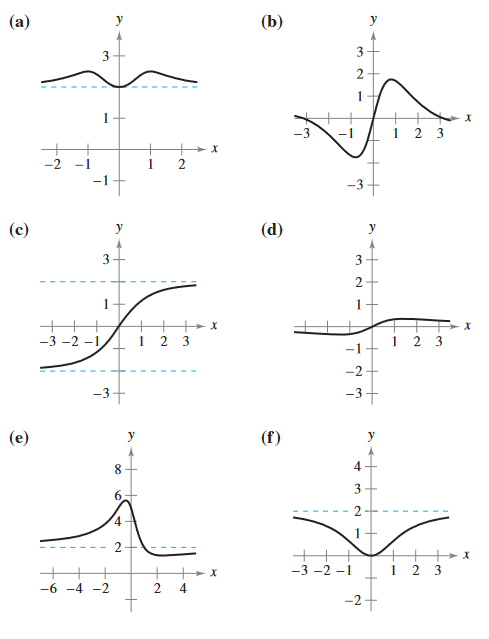
\includegraphics[scale=0.75]{4.png}\\
2.\[f(x)=\frac{2x}{\sqrt[]{x^2+2}}\]
The function has a horizontal asymptote at $y=\pm 2$. Therefore, it matches (c). 

\vs\next
4.\[f(x)=2+\frac{x^2}{x^4+1}\]
The function has a vertical asymptote at $y=2$. Therefore, it matches (a).

\vs\next
6.\[f(x)=\frac{2x^2-3x+5}{x^2+1}\]
The function has a horizontal asymptote at $y=2$. Therefore, it matches (e).

\section{Use a graphing utility to complete the table and estimate the limit as $x$ approaches infinity. Then use a graphing utility to graph the funciton and estimate the limit graphically.}
8.\[f(x)=\frac{2x^2}{x+1}\]
\begin{flushleft}
    \begin{table}[h]
        \begin{tabular}{|l|l|l|l|l|l|l|l|}
        \hline
        $x$ & $10^0$ & $10^1$ & $10^2$ & $10^3$ & $10^4$ & $10^5$ & $10^6$\\ \hline
        $f(x)$ & $1$ & $18.18$ & $198.02$ & $1998.02$ & $19998$ & $199998$ & $1999998$\\ \hline
        \end{tabular}
    \end{table}
\end{flushleft}
$\lim_{x\to\infty}f(x)=\infty\therefore$ it doesn't exist.

12.\[f(x)=4+\frac{3}{x^2+2}\]
\begin{flushleft}
    \begin{table}[h]
        \begin{tabular}{|l|l|l|l|l|l|l|l|}
        \hline
        $x$ & $10^0$ & $10^1$ & $10^2$ & $10^3$ & $10^4$ & $10^5$ & $10^6$\\ \hline
        $f(x)$ & $5$ & $4.03$ & $4.0003$ & $4$ & $4$ & $4$ & $4$\\ \hline
        \end{tabular}
    \end{table}
\end{flushleft}
$\lim_{x\to\infty}f(x)=4$

\section{Find $\lim_{x\to\infty}h(x)$, if possible.}
14.\[f(x)=-4x^2+2x-5\]
\begin{enumerate}[(a)]
    \item $h(x)=\frac{f(x)}{x}$
        \begin{align}
            &=\frac{-4x^2+2x-5}{x}\\
            &=-4x+2-\frac{5}{x}\\
            \lim_{x\to\infty}h(x)&=-\infty\therefore\,\,\text{the limit doesn't exist.}
        \end{align}
    \item $h(x)=\frac{f(x)}{x^2}$
        \begin{align}
            \set
            &=\frac{-4x^2+2x-5}{x^2}\\
            &=-4+\frac{2}{x}-\frac{5}{x^2}\\
            \lim_{x\to\infty}h(x)&=-4
        \end{align}
    \item $h(x)=\frac{f(x)}{x^3}$
        \begin{align}
            \set
            &=\frac{-4x^2+2x-5}{x^3}\\
            &=-\frac{4}{x}+\frac{2}{x^2}-\frac{5}{x^3}\\
            \lim_{x\to\infty}h(x)&=0
        \end{align}
\end{enumerate}

\section{Find each limit, if possible.}
18.\begin{enumerate}[(a)]
    \item \[\lim_{x\to\infty}\frac{5x^{3/2}}{4x^2+1}=0\]
    \item \[\lim_{x\to\infty}\frac{5x^{3/2}}{4x^{3/2}+1}=\frac{5}{4}\]
    \item \[\lim_{x\to\infty}\frac{5x^{3/2}}{4\sqrt[]{x}+1}=\infty\therefore\text{the limit doesn't exist.}\]
    \item 
\end{enumerate}

\section{Find the limit}
22.\[\lim_{x\to\infty}\frac{x^2+3}{2x^2-1}\]
\begin{align}
    \set
    &=\lim_{x\to\infty}\frac{1+\frac{3}{x^2}}{2-\frac{1}{x}}\\
    &=\frac{1+0}{2-0}\\
    &=\frac{1}{2}
\end{align}

\vs\next
24.\[\lim_{x\to\infty}\frac{5x^3+1}{10x^3-3x^2+7}\]
\begin{align}
    \set
    &=\lim_{x\to\infty}\frac{5+\frac{1}{x^3}}{10-\frac{3}{x}+\frac{7}{x^3}}\\
    &=\frac{5+0}{10-0}\\
    &=\frac{1}{2}
\end{align}

\vs\next
28.\[\lim_{x\to-\infty}\frac{x}{\sqrt[]{x^2+1}}\]
\begin{align}
    \set
    &=\lim_{x\to-\infty}\frac{1}{\left(\frac{\sqrt[]{x^2+1}}{-\sqrt[]{x^2}}\right)}\\
    &=\lim_{x\to-\infty}\frac{-1}{\sqrt[]{1+\frac{1}{x^2}}}=-1
\end{align}

\vs
\next
32.\[\lim_{x\to\infty}\frac{\sqrt[]{x^4-1}}{x^3-1}\]
\begin{align}
    \set
    &=\lim_{x\to\infty}\frac{\sqrt[]{x^4-1}}{x^3-1}\left(\frac{\frac{1}{-\sqrt[]{x^6}}}{\frac{1}{x^3}}\right)\\
    &=\lim_{x\to\infty}\frac{\sqrt[]{\frac{1}{x^2}-\frac{1}{x^6}}}{-1+\frac{1}{x^3}}\\
    &=0
\end{align}

\vs\next
36.\[\lim_{x\to\infty}\cos\frac{1}{x}\]
\begin{align}
    \set
    &=\cos 0\\
    &=1
\end{align}

\section{Use a graphing utility to graph the function and identify any horizontal asymptotes.}
40.\[f(x)=\frac{|3x+2|}{x-2}\]
$y=3$ is a horizontal asymptote from the right and $y=-3$ from the left.

\vs
\next
42.\[f(x)=\frac{\sqrt[]{9x^2-2}}{2x+1}\]
$y=\frac{3}{2}$ is a horizontal asymptote from the right and $y=-\frac{3}{2}$ from the left.

\section{Find the limit.}
44.\[\lim_{x\to\infty}x\tan\frac{1}{x}\]
Let $x=\frac{1}{t}$
\begin{align}
    \set
    &=\lim_{x\to 0^+}\frac{\tan t}{t}\\
    &=\lim_{x\to 0^+}\left(\frac{\sin t}{t}\cdot\frac{1}{\cos t}\right)\\
    &=(1)(1)
    &=1
\end{align}

48.\[\lim_{x\to\infty}(4x-\sqrt[]{16x^2-x})\]
\begin{align}
    \set
    &=\lim_{x\to\infty}(4x-\sqrt[]{16x^2-x})\frac{4x-\sqrt[]{16x^2-x}}{4x-\sqrt[]{16x^2-x}}\\
    &=\lim_{x\to\infty}\frac{16x^2-(16x^2-x)}{4x+\sqrt[]{(16x^2-x)}}\\
    &=\lim_{x\to\infty}\frac{x}{4x+\sqrt[]{16x^2-x}}\\
    &=\lim_{x\to\infty}\frac{1}{4+\sqrt[]{16x^2-x}}\\
    &=\frac{1}{4+4}
    &=\frac{1}{8}
\end{align}

\section{Use a graphing utility to complete the table and estimate the limit as $x$ approaches infinity. Then user a graphing utility to graph the function and estimate the limit. Finally, find the limit analitically and compare your results with the estimates.}
52.\[f(x)=\frac{x+1}{x\sqrt[]{x}}\]
\begin{flushleft}
    \begin{table}[h]
        \begin{tabular}{|l|l|l|l|l|l|l|l|}
        \hline
        $x$ & $10^0$ & $10^1$ & $10^2$ & $10^3$ & $10^4$ & $10^5$ & $10^6$\\ \hline
        $f(x)$ & $2$ & $0.348$ & $0.101$ & $0.032$ & $0.010$ & $0.003$ & $0.001$\\ \hline
        \end{tabular}
    \end{table}
\end{flushleft}
\[\lim_{x\to\infty}\frac{x+1}{x\sqrt[]{x}}=0\]

\section{Describe in your own words what the statement means.}
54.\[\lim_{x\to-\infty}f(x)=2\]
It means that the function approaches 2 as $x$ becomes an infinite and negative value.

\section{Capstone}
58. The graph of a function $f$ is shown below.\\
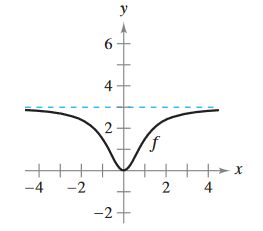
\includegraphics{58a.png}
\begin{enumerate}[(a)]
    \item Sketch $f'$\\ 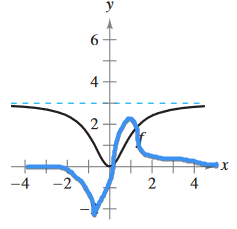
\includegraphics{58b.png}
    \item Use the graphs to estimate $\lim_{x\to\infty}f(x)$ and $\lim_{x\to\infty}f'(x)$.\\
    \[\lim_{x\to\infty}f(x)=3\] and \[\lim_{x\to\infty}f'(x)=0\]
    \item Because the first limit approaches a constant, we can deduce that the graph is approaching that of a line with slope of zero: a horizontal line.
\end{enumerate}

\section{Sketch the graph of the equation using extrema, intercepts, symmetry and asymptotes. The use a graphing utility to verify your result.}
60.\[y=\frac{x-4}{x-3}\]
\begin{enumerate}
    \item Intercepts: $(0, \frac{4}{3})$, $(4, 0)$
    \item No symmetry
    \item Horizontal asymptotes: $y=1$
    \item Vertical asymptotes: $x=3$
\end{enumerate}
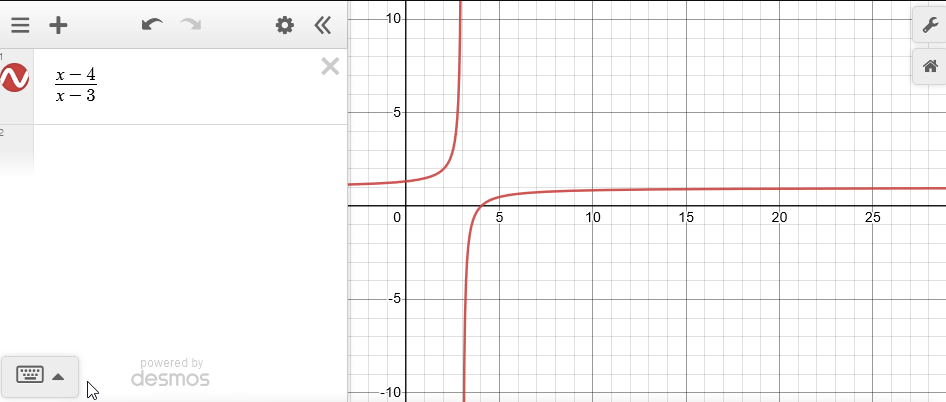
\includegraphics[scale=0.5]{60.png}

64.\[y=\frac{x^2}{x^2-16}\]
\begin{enumerate}
    \item Intercepts: $(0, 0)$
    \item Symmetry in the y-axis
    \item Horizontal asymptotes: $y=1$
    \item Vertical asymptotes: $x=\pm 4$
    \item $y'=\frac{-32x}{(x^2-16)^2}$
    \item Relative maxima: (0, 0)
\end{enumerate}
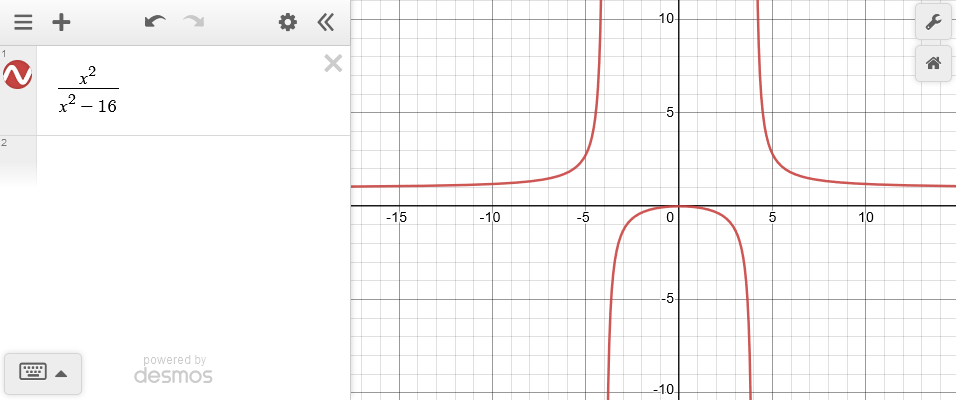
\includegraphics[scale=0.5]{61.png}

72.\[y=\frac{1}{x}\]
\begin{enumerate}
    \item Intercepts: $(-1, 0)$
    \item No symmetry
    \item Horizontal asymptotes: $y=1$
    \item Vertical asymptotes: $x=0$
\end{enumerate}
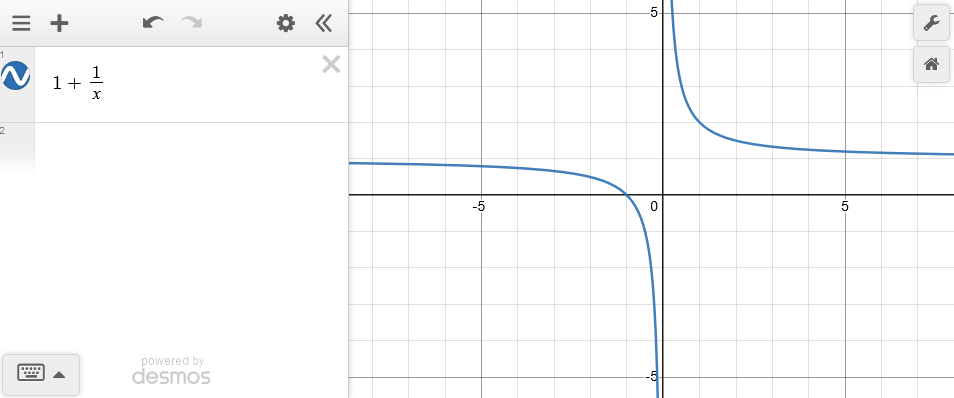
\includegraphics[scale=0.5]{72.png}

\section{(a) Use a graphing utility to graph $f$ and $g$ in the same viewing window, (b) verify algebraically that $f$ and $g$ represent the same function, and (c) zoom out sufficiently far so that the graph appears as a line. What equation does this line appear to have? (Note that the points at which function is not continuous are not readily seen when you zoom out.)}
86.\[f(x)=-\frac{x^3-2x^2+2}{2x^2}\]
\[g(x)=-\frac{1}{2}x+1-\frac{1}{x^2}\]
\begin{enumerate}
    \item[(b)] \begin{align}
        \set
        f(x)&=-\frac{x^3-2x^2+2}{2x^2}\\
        &=-\left(\frac{x^3}{2x^2}-\frac{2x^2}{2x^2}+\frac{2}{2x^2}\right)\\
        &=-\frac{1}{2}x+1-\frac{1}{x^2}\\
        &=g(x)
    \end{align}
    \item[(c)] The graph appears to be the line $y=-\frac{1}{2}+1$
\end{enumerate}

\section{Word problems}
88. A business has a cost of $C=0.5x+500$ for producing $x$ units. The average cost per unit is $\overline{C}=\frac{C}{x}$. Find the limit of $\overline{C}$ as $x$ approaches infinity.
\begin{align}
    \set
    \overline{C}&=0.5+\frac{500}{x}\\
    \lim_{x\to\infty}&\left(0.5+\frac{500}{x}\right)=0.5
\end{align}

\vs\next
90. The graph shows the temperature $T$, in degrees Fahrenheit, of molten glass $t$ seconds after it is removed from a kiln.\\
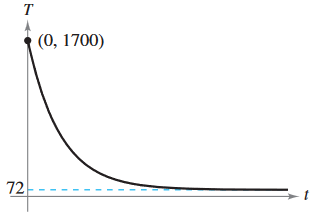
\includegraphics{90.png}
\begin{enumerate}[(a)]
    \item Find $\lim_{t\to 0^+}T$. What does this limit represent?\\
    \indent The temperature of the kiln.
    \item Find $\lim_{t\to\infty}T$. What does this limit represent?\\
    \indent The room's temperature.
    \item Will the temperature of the glass ever actually reach room temperature? Why?\\
    \indent No because $y=72$ is a horizontal asymptote.
\end{enumerate}

\vs\next
92. The average typing speeds $S$ (in words per minute) of a typing student after $t$ weeks of lessons are shown in the table.\\
 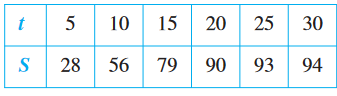
\includegraphics{92.png}\\
 A model for the data is $S=\frac{100t^2}{65+t^2},\,\,\, t>0$
 \begin{enumerate}[(a)]
    \item Use a graphing utility to plot the data and graph the model.
    \item Does there appear to be a limiting typing speed? Explain.\\
    \indent Yes because $\lim_{t\to\infty}S=\frac{100}{1}=100$. 
 \end{enumerate}

 \vs\next
 96. A line with slope $m$ passes through the point (0, -2).
 \begin{enumerate}[(a)]
    \item Write the distance $d$ between the line and the point (4, 2) as a function of $m$.\\
    Rewriting the line's equation:
    \begin{align}
        \set
        y+2=m(x-0)\\
        mx-y-2=0
    \end{align}
    Finding the function:
    \begin{align}
        d&=\frac{|Ax_1+By_1+C|}{\sqrt[]{A^2+B^2}}\\
        &=\frac{|m(4)-1(2)-2|}{\sqrt[]{m^2+1}}\\
        &=\frac{|4m-4|}{\sqrt[]{m^2+1}}
    \end{align}
    \item Use a graphing utlity to graph the equation in part (a).
    \item Find $\lim_{m\to\infty}d(m)$ and $\lim_{m\to-\infty}d(m)$. Interpret the results geometrically.
    \[\lim_{m\to\infty}d(m)=4;\,\,\,\,\lim_{m\to-\infty}d(m)=4\]
The distance from the given point approaches 4 because the line approaches the origin's vertical line $x=0$.
\end{enumerate}

\section{Use the definition of limits at infinity to prove the limit.}
104.\[\lim_{x\to-\infty}\frac{1}{x-2}=0\]
Let $\epsilon>0$. We are finding $N<0$ such that $|f(x)-L|=\frac{-1}{x-2}<\epsilon$ when $x<N$
\begin{align}
    \set
    \frac{-1}{x-2}<\epsilon\Rightarrow x-2<\frac{-1}{\epsilon}\Rightarrow x<2-\frac{1}{\epsilon}\\
    x<N=2-\frac{1}{\epsilon}\\
    x-2<\frac{-1}{\epsilon}\\
    \frac{-1}{x-2}<\epsilon\\
    \Rightarrow|f(x)-L|<\epsilon
\end{align}

\section{Determine whether the statement is true or false. If it is false, explain why or give an example that shows it is false.}
107. If $f'(x)>0$ for all real numbers $x$, then $f$ increases without bound.\\
\indent False. $f(x)=\frac{2x}{\sqrt[]{x^2+2}}$ from Exercise 54 proves otherwise.

\vs\next
108. If $f''(x)$ for all real numbers $x$, then $f$ decreases without bound.\\
\indent False. $f(x)=-x^2$ increases without bound even though $f''(x)=-2<0,\,\, x\in\mathbb{R}$.












\end{document}